\section{IVM for the Relational Algebra}\label{sec:relational}

Results in \secref{sec:streams} and~\secref{sec:incremental}
apply to streams of arbitrary group values.  In this
section we use these results in the context of IVM for
relational databases.  As explained in the introduction, our goal is to
efficiently compute the incremental version of any relational query $Q$
that defines a database view.

However, we face a technical problem: the $\I$ and $\D$ operators were
defined on abelian groups, and relational databases in general are 
not abelian groups, since they operate on sets.  Fortunately, 
there is a well-known tool in the database literature
which converts set operations into group operations by using \zrs
(also called z-relations elsewhere~\cite{green-tcs11}) instead of sets.

We start by defining the \zrs group, and then we review how 
relational queries are converted into \dbsp circuits  over \zrs.  
This translation is efficiently incrementalizable because
many basic relational queries can be expressed using LTI \zr operators~\refsec{sec:relational-operators}.

\subsection{\zrs as an abelian group}

Given a set $A$, we define \defined{\zrs} 
over $A$ as functions with \emph{finite support} from $A$ to $\Z$.  
These are functions $f: A \rightarrow \Z$ where 
$f(x) \not= 0$ for at most a finite number of values $x \in A$.
We also write $\Z[A]$ for the type of \zrs with elements from $A$.
Values in $\Z[A]$ can be thought of as key-value maps with 
keys in $A$ and values in $\Z$, justifying the array indexing notation.  
If $m \in \Z[A]$ we write $m[a]$ instead of $m(a)$, again using
an indexing notation.  

A particular \zr $m \in \Z[A]$ can be denoted by enumerating its
elements that have non-zero values and their corresponding values: 
$m = \{ x_1 \mapsto w_1, \dots, x_n \mapsto w_n \}$.  
We call $w_i \in \Z$ the \defined{multiplicity} (or weight)
of $x_i \in A$.  Multiplicities can be negative.  
We write that $x \in m$ iff $m[x] \not= 0$.
In terms of databases think of a \zr as a table
where each row as an associated weight, possibly negative.
We also write $w \cdot x$ for $\{ x \mapsto w \}$.

\ifzsetexamples
Consider a concrete \zr $R \in \Z[\texttt{string}]$,
defined by $R = \{ \texttt{joe} \mapsto 1, \texttt{anne} \mapsto -1 \}$.  
$R$ has two elements in its domain,
\texttt{joe} with a multiplicity of 1 (so $R[\texttt{joe}] = 1$), 
and \texttt{anne} with a multiplicity of $-1$.
We say \texttt{joe} $\in R$ and \texttt{anne} $\in R$.
\fi

Since $\Z$ is an abelian ring, $\Z[A]$ is also an abelian ring (and thus a group).  This group
$(\Z[A], +_{\Z[A]}, 0_{\Z[A]}, -_{\Z{A}})$ has addition and subtraction defined pointwise: 
$(f +_{\Z[A]} g)(x) = f(x) + g(x) . \forall x \in A.$  
The $0$ element of $\Z[A]$ is the function $0_{\Z[A]}$ defined by $0_{\Z[A]}(x) = 0 . 
\forall x \in A$.  For example $R + R =  \{ \texttt{joe} \mapsto 2, \texttt{anne} \mapsto -2 \}$.
Since \zrs form a group, all the results from \secref{sec:streams} apply to streams over \zrs. 

\zrs generalize sets and bags.  A set with elements from $A$
can be represented as a \zr by associating a weight of 1 with each element.
Bags are \zrs where all weights are positive.  Crucially, \zrs
can also represent arbirary \emph{changes} to sets and bags.
Negative weights in a change represent elements that are being ``removed''.

\begin{definition}
We say that a \zr represents a \defined{set} if the multiplicity of every
element is one.  We define a function to check this property 
$\isset : \Z[A] \rightarrow \B$\index{isset}
given by:
$$\isset(m) \defn \left\{
\begin{array}{ll}
  \mbox{true} & \mbox{ if } m[x] = 1, \forall x \in m \\
  \mbox{false} & \mbox{ otherwise}
\end{array}
\right.
$$
\end{definition}

\ifzsetexamples
For our example $\isset(R) = \mbox{false}$, since $R[\texttt{anne}] = -1$.  
\fi

\begin{definition}
We say that a \zr is \defined{positive} (or a \defined{bag}) if the multiplicity of every element is
positive.  We define a function to check this property
$\ispositive : \Z[A] \rightarrow \B$\index{ispositive}.
given by
$$\ispositive(m) \defn \left\{
\begin{array}{ll}
  \mbox{true} & \mbox{ if } m[x] \geq 0, \forall x \in A \\
  \mbox{false} & \mbox{ otherwise}
\end{array}
\right.$$
$\forall m \in \Z[A] . \isset(m) \Rightarrow \ispositive(m)$.
\end{definition}

\ifzsetexamples
We have $\ispositive(R) = \mbox{false}$, since $R[\texttt{anne}] = -1$.
\fi

We write $m \geq 0$ when $m$ is
positive.  For positive $m, n$ we write $m \geq n$ for $m, n
\in \Z[A]$ iff $m - n \geq 0$.  $\geq$ is a partial order.

We call a function $f : \Z[A] \rightarrow \Z[B]$ \defined{positive} if it maps
positive values to positive values:
$\forall x \in \Z[A], x \geq 0_{\Z[A]} \Rightarrow f(x) \geq 0_{\Z[B]}$.  
We apply this notation to functions as well: $\ispositive(f)$.

\begin{definition}[distinct]
The function $\distinct: \Z[A] \rightarrow \Z[A]$\index{distinct}
``converts'' a \zr into a set:
$$\distinct(m)[x] \defn \left\{
\begin{array}{ll}
  1 & \mbox{ if } m[x] > 0 \\
  0 & \mbox{ otherwise}
\end{array}
\right.
$$
\end{definition}

Notice that $\distinct$ ``removes'' duplicates from multisets, and it also eliminates 
elements with negative multiplicities.
\ifzsetexamples
$\distinct(R) = \{ \texttt{joe} \mapsto 1 \}$.
\fi
While very simple, this definition of $\distinct$ has been carefully 
chosen to enable us to implement the relational (set) operators
using \zrs operators.
Circuits derived from relational queries only compute on positive \zrs.

\begin{definition}(mononotonicity)
A stream $s \in \stream{\Z[A]}$ is \defined{positive} if every value of the stream is positive:
$s[t] \geq 0 . \forall t \in \N$.
A stream $s \in \stream{\Z[A]}$ is \defined{monotone} if $s[t] \geq s[t-1], \forall t \in \N$.
\end{definition}

If $s \in \stream{\Z[A]}$ is positive, then $\I(s)$ is monotone.
If $s \in \stream{\Z[A]}$ is monotone, $\D(s)$ is positive.

\paragraph{Generalizing circuit diagrams}

From now on we will use circuits to compute both on scalars (\zrs in our case) and streams of \zrs.
We use the same graphical representation for functions on streams or scalars: 
boxes with input and output arrows.  For scalar functions the ``values'' 
of the arrows are scalars instead of streams; otherwise
the interpretation of boxes as function application is unchanged.  We will
thus use circuits to depict relational query plans.

\subsection{Implementing relational operators}\label{sec:relational-operators}

The fact that relational algebra can be implemented by computations
on \zrs has been shown before, e.g.~\cite{green-pods07}.  The translation
of the relational operators to \dbsp is shown in Table~\ref{tab:relational}.  
The first row of the table shows that a composite query is translated
recursively.  This gives us a recipe for
translating an arbitrary relational query plan into a \dbsp circuit.

\newlength{\commentsize}
\setlength{\commentsize}{5cm}
\begin{table*}[h]
\small
\begin{tabular}{|m{1.2cm}m{4.2cm}m{5cm}m{\commentsize}|} \hline
Operation & SQL example & \dbsp circuit & Details \\ \hline
Composition &
 \begin{lstlisting}[language=SQL]
SELECT DISTINCT ... FROM 
(SELECT ... FROM ...)
\end{lstlisting}
 & 
 \begin{tikzpicture}[auto,>=latex]
  \node[] (I) {\code{I}};
  \node[block, right of=I] (CI) {$C_I$};
  \draw[->] (I) -- (CI);
  \node[block, right of=CI] (CO) {$C_O$};
  \node[right of=CO] (O) {\code{O}};
  \draw[->] (CI) -- (CO);
  \draw[->] (CO) -- (O); 
\end{tikzpicture}
 &
 \parbox[b][][t]{\commentsize}{
  $C_I$ circuit for inner query, \\
  $C_O$ circuit for outer query.}  
\\ \hline
Union & 
\begin{lstlisting}[language=SQL]
(SELECT * FROM I1) 
UNION 
(SELECT * FROM I2)
\end{lstlisting}
&
\begin{tikzpicture}[auto,>=latex]
  \node[] (input1) {\code{I1}};
  \node[below of=input1, node distance=.4cm] (midway) {};
  \node[below of=midway, node distance=.4cm] (input2) {\code{I2}};
  \node[block, shape=circle, right of=midway, inner sep=0in] (plus) {$+$};
  \node[block, right of=plus] (distinct) {$\distinct$};
  \node[right of=distinct] (output) {\code{O}};
  \draw[->] (input1) -| (plus);
  \draw[->] (input2) -| (plus);
  \draw[->] (plus) -- (distinct);
  \draw[->] (distinct) -- (output);
\end{tikzpicture}
&
\\ \hline
Projection &
\begin{lstlisting}[language=SQL]
SELECT DISTINCT I.c 
FROM I
\end{lstlisting}
&
\begin{tikzpicture}[auto,>=latex]
  \node[] (input) {\code{I}};
  \node[block, right of=input] (pi) {$\pi$};
  \node[block, right of=pi] (distinct) {$\distinct$};
  \node[right of=distinct] (output) {\code{O}};
  \draw[->] (input) -- (pi);
  \draw[->] (pi) -- (distinct);
  \draw[->] (distinct) -- (output);
\end{tikzpicture}
&
\parbox[b][][t]{\commentsize}{
$\pi(i)[y] \defn
\sum_{x \in i, x|_c = y} i[x]$ \\
$x|_c$ is projection on column $c$ of the tuple $x$ \\
$\pi$ is linear; $\ispositive(\pi), \zpp{\pi}$.
}
\\ \hline
Filtering &
\begin{lstlisting}[language=SQL]
SELECT * FROM I 
WHERE p(I.c)
\end{lstlisting}
&
\begin{tikzpicture}[auto,>=latex]
  \node[] (input) {\code{I}};
  \node[block, right of=input] (map) {$\sigma_P$};
  \node[right of=map] (output) {\code{O}};
  \draw[->] (input) -- (map);
  \draw[->] (map) -- (output);
\end{tikzpicture}
&
\parbox[b][][t]{\commentsize}{
$\sigma_P(m)[x] \defn \left\{
\begin{array}{ll}
  m[x] \cdot x & \mbox{ if } P(x) \\
  0 & \mbox{ otherwise } \\
\end{array}
\right.$ \\
$P: A \rightarrow \B$ is a predicate. \\
$\sigma_P$ is linear; $\ispositive(\sigma_P), \zpp{\sigma_P}$.
}
% \\ \hline
%Selection &
%\begin{lstlisting}[language=SQL]
%SELECT DISTINCT f(I.c, ...) 
%FROM I
%\end{lstlisting}
%&
%\begin{tikzpicture}[auto,>=latex]
%  \node[] (input) {\code{I}};
%  \node[block, right of=input, node distance=1.5cm] (map) {$\mbox{map}(f)$};
%  \node[block, right of=map, node distance=1.5cm] (distinct) {$\distinct$};
%  \node[right of=distinct, node distance=1.5cm] (output) {\code{O}};
%  \draw[->] (input) -- (map);
%  \draw[->] (map) -- (distinct);
%  \draw[->] (distinct) -- (output);
%\end{tikzpicture}
%& 
%\parbox[b][][t]{\commentsize}{
%For a function $f$ \\
%$\map(f)$ is linear, \\
%$\ispositive(\map(f)), \zpp{\map(f)}$
%}.
\\ \hline
\parbox[b][][t]{1cm}{
Cartesian \\
product} &
\begin{lstlisting}[language=SQL]
SELECT I1.*, I2.* 
FROM I1, I2
\end{lstlisting}
& 
\begin{tikzpicture}[auto,>=latex]
  \node[] (i1) {\code{I1}};
  \node[below of=i1, node distance=.4cm] (midway) {};
  \node[below of=midway, node distance=.4cm] (i2) {\code{I2}};
  \node[block, right of=midway] (prod) {$\times$};
  \node[right of=prod] (output) {\code{O}};
  \draw[->] (i1) -| (prod);
  \draw[->] (i2) -| (prod);
  \draw[->] (prod) -- (output);
\end{tikzpicture}
& 
\parbox[b][][t]{\commentsize}{
$(a \times b)((x,y)) \defn a[x] \times b[y]$. \\
$\times$ is bilinear, $\ispositive(\times), \zpp{\times}$.
}
\\ \hline
Equi-join &
\begin{lstlisting}[language=SQL]
SELECT I1.*, I2.* 
FROM I1 JOIN I2
ON I1.c1 = I2.c2
\end{lstlisting}
&
\begin{tikzpicture}[auto,>=latex]
  \node[] (i1) {\code{I1}};
  \node[below of=i1, node distance=.4cm] (midway) {};
  \node[below of=midway, node distance=.4cm] (i2) {\code{I2}};
  \node[block, right of=midway] (prod) {$\bowtie_{c1 = c2}$};
  \node[right of=prod] (output) {\code{O}};
  \draw[->] (i1) -| (prod);
  \draw[->] (i2) -| (prod);
  \draw[->] (prod) -- (output);
\end{tikzpicture}
&
\parbox[b][][t]{\commentsize}{
$(a \bowtie b)((x,y)) \defn a[x] \times b[y] \\
\mbox{ if } x|_{c1} = y|_{c2}$. \\
$\bowtie$ is bilinear, $\ispositive(\bowtie), \zpp{\bowtie}$.
}
\\ \hline
Intersection &
\begin{lstlisting}[language=SQL]
(SELECT * FROM I1)
INTERSECT 
(SELECT * FROM I2)
\end{lstlisting}
&
\begin{tikzpicture}[auto,>=latex]
  \node[] (i1) {\code{I1}};
  \node[below of=i1, node distance=.4cm] (midway) {};
  \node[below of=midway, node distance=.4cm] (i2) {\code{I2}};
  \node[block, right of=midway] (prod) {$\bowtie$};
  \node[right of=prod] (output) {\code{O}};
  \draw[->] (i1) -| (prod);
  \draw[->] (i2) -| (prod);
  \draw[->] (prod) -- (output);
\end{tikzpicture}
&
Special case of equi-join when both relations have the same schema.
 \\ \hline
Difference &
\begin{lstlisting}[language=SQL]
SELECT * FROM I1 
EXCEPT 
SELECT * FROM I2
\end{lstlisting}
&
\begin{tikzpicture}[auto,>=latex, node distance=.7cm]
  \node[] (i1) {\code{I1}};
  \node[below of=i1, node distance=.4cm] (midway) {};
  \node[below of=midway, node distance=.4cm] (i2) {\code{I2}};
  \node[block, shape=circle, inner sep=0in, right of=i2] (m) {$-$};
  \node[block, right of=midway, shape=circle, inner sep=0in, node distance=1.3cm] (plus) {$+$};
  \node[block, right of=plus, node distance=1cm] (distinct) {$\distinct$};
  \node[right of=distinct, node distance=1cm] (output) {\code{O}};
  \draw[->] (i1) -| (plus);
  \draw[->] (i2) -- (m);
  \draw[->] (m) -| (plus);
  \draw[->] (plus) -- (distinct);
  \draw[->] (distinct) -- (output);
\end{tikzpicture}
&
\\ \hline
\end{tabular}
\caption{Implementation of SQL relational set operators in \dbsp.  
Each query assumes that inputs \code{I}, \code{I1}, \code{I2}, are sets and it 
produces output sets.\label{tab:relational}}
\end{table*}


The translation is fairly straightforward, but many operators require
the application of a $\distinct$ to produce sets.  
For example, $a \cup b = \distinct(a + b)$, $a \setminus b = 
\distinct(a - b)$, $(a \times b)((x,y)) = a[x] \times b[y]$.

\paragraph{Correctness of the \dbsp implementations}\label{sec:correctness}

A relational query $Q$ that transforms
a set $V$ into a set $U$ is implemented by a \dbsp computation $Q'$ on 
\zrs.  The correctness of the implementation requires the following
diagram to commute:

\begin{center}
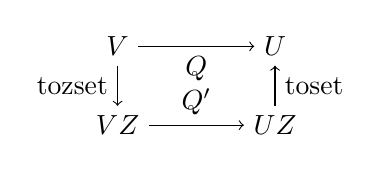
\begin{tikzpicture}
  \node[] (V) {$V$};
  \node[below of=V] (VZ) {$VZ$};
  \node[right of=V, node distance=2cm] (U) {$U$};
  \node[below of=U] (UZ) {$UZ$};
  \draw[->] (V) -- node (f) [below] {$Q$} (U);
  \draw[->] (V) --  node (s) [left] {tozset}(VZ);
  \draw[->] (VZ) -- node (f) [above] {$Q'$} (UZ);
  \draw[->] (UZ) -- node (d) [right] {toset} (U);
\end{tikzpicture}
\end{center}

(The correctness of
this implementation is predicated on $Q'$'s inputs being
sets, an invariant which needs to be maintained by the environment.) 
The ``$\mbox{toset}$'' and ``$\mbox{tozset}$'' functions convert sets to \zrs and 
vice-versa, in the expected way:

$\mbox{toset}: \Z[A] \to 2^A$ is defined as $\mbox{toset}(m) \defn \cup_{x \in \distinct(m)} \{ x \}$.

$\mbox{tozset}: 2^A \to \Z[A]$ is defined as $\mbox{tozset}(s) \defn \sum_{x \in s} 1 \cdot x$.

%All standard algebraic properties
%of the relational operators can be used to optimize circuits
%(they can even be applied to queries before building the circuits).

Notice that the use of the $\distinct$ operator allows \dbsp to model
the \emph{full relational algebra}, including set difference (and not just the positive
fragment).  Prior work (e.g., Proposition 6.13 in~\cite{green-tcs11}) has shown
how some invocations of $\distinct$ can be eliminated from query plans 
without changing the query semantics.

\begin{proposition}\label{prop-distinct-delay}
Let $Q$ be one of the following \zrs operators: filtering $\sigma$,
join $\bowtie$, or Cartesian product $\times$.
Then we have $\forall i \in \Z[I], \ispositive(i) \Rightarrow Q(\distinct(i)) = \distinct(Q(i))$.
\end{proposition}

\begin{comment}
\noindent
\begin{tabular}{m{3.5cm}m{.5cm}m{3.5cm}}
\begin{tikzpicture}[auto,>=latex]
  \node[] (input) {$i$};
  \node[block, right of=input, node distance=1.1cm] (distinct) {$\distinct$};
  \node[block, right of=distinct, node distance=1.2cm] (q) {$Q$};
  \node[right of=q] (output)  {$o$};
  \draw[->] (input) -- (distinct);
  \draw[->] (distinct) -- (q);
  \draw[->] (q) -- (output);
\end{tikzpicture}
&
$\cong$
&
\begin{tikzpicture}[auto,>=latex]
  \node[] (input) {$i$};
  \node[block, right of=input] (q) {$Q$};
  \node[block, right of=q, node distance=1.2cm] (distinct1) {$\distinct$};
  \node[right of=distinct1, node distance=1.2cm] (output)  {$o$};
  \draw[->] (input) -- (q);
  \draw[->] (q) -- (distinct1);
  \draw[->] (distinct1) -- (output);
\end{tikzpicture}
\end{tabular}

This rule allows us to delay the application of $\distinct$.
\end{comment}

\begin{proposition}\label{prop-distinct-once}
Let $Q$ be one of the following \zrs operators: filtering $\sigma$,
projection $\pi$, map($f$)\footnote{Technically map (applying a user-defined
function to each row in a table) is not a relational operator.},
addition $+$, join $\bowtie$, or
Cartesian product $\times$.
Then we have $\ispositive(i) \Rightarrow \distinct(Q(\distinct(i))) = \distinct(Q(i))$.
\end{proposition}

\begin{comment}
\noindent
\begin{tabular}{m{6.5cm}m{.5cm}}
\begin{tikzpicture}[auto,>=latex]
  \node[] (input) {$i$};
  \node[block, right of=input, node distance=1.5cm] (distinct) {$\distinct$};
  \node[block, right of=distinct, node distance=1.5cm] (q) {$Q$};
  \node[block, right of=q, node distance=1.5cm] (distinct1) {$\distinct$};
  \node[right of=distinct1, node distance=1.5cm] (output)  {$o$};
  \draw[->] (input) -- (distinct);
  \draw[->] (distinct) -- (q);
  \draw[->] (q) -- (distinct1);
  \draw[->] (distinct1) -- (output);
\end{tikzpicture}
&
$\cong$ \\
\begin{tikzpicture}[auto,>=latex]
  \node[] (input) {$i$};
  \node[block, right of=input] (q) {$Q$};
  \node[block, right of=q, node distance=1.5cm] (distinct1) {$\distinct$};
  \node[right of=distinct1, node distance=1.5cm] (output)  {$o$};
  \draw[->] (input) -- (q);
  \draw[->] (q) -- (distinct1);
  \draw[->] (distinct1) -- (output);
\end{tikzpicture}
\end{tabular}
\end{comment}

These properties allow us to ``consolidate'' distinct operators by performing
one $\distinct$ at the end of a chain of computations.

\subsection{Incremental view maintenance}

Let us consider a relational query $Q$ 
defining a view $V$.  To create a circuit that maintains incrementally $V$
we apply the following mechanical steps (this algorithm is deterministic
and its running time is proportional to the number of operators in the query):

\begin{algorithm}[incremental view maintenance]\label{algorithm-inc}\quad
\begin{enumerate}[nosep, leftmargin=\parindent]
    \item Translate $Q$ into a circuit using the rules in Table~\ref{tab:relational}.
    \item Apply $\distinct$ elimination rules (\ref{prop-distinct-delay}, \ref{prop-distinct-once}) until convergence\footnote{The 
    order in which the rules are applied does not matter, since the algorithm is 
    confluent: it always produces the same final result. So the rules can be applied in topological order.}.
    \item Lift the whole circuit, by applying Proposition~\ref{prop:distributivity},
    converting it to a circuit operating on streams.
    \item Incrementalize the whole circuit ``surrounding'' it with $\I$ and $\D$.
    \item Apply the chain rule 
    from Proposition~\ref{prop-inc-properties} recursively on the query structure
    to obtain an incremental implementation.  
\end{enumerate}
\end{algorithm}

A query can be implemented by multiple plans, with varying data-dependent costs.  The input provided
to this algorithm is a standard relational query plan, and this algorithm produces
an incremental plan that is ``similar'' to the input plan\footnote{Query planners generally use cost-based 
heuristics to optimize plans, but IVM planning in general does not have this luxury, since the plan
must be generated \emph{before} the data has been fed to the database.  Nevertheless, standard query 
optimization techniques, perhaps based on historical statistics, can be applied to the query plan before 
generating the incremental plan.}.  Step (2) generates an equivalent circuit, with possibly 
fewer $\distinct$ operators.
Step (3) yields a circuit that consumes a \emph{stream} of complete database snapshots and outputs a 
stream of complete view snapshots. Step (4) yields a circuit that consumes a stream of \emph{database changes}
and outputs a stream of \emph{view changes}; however, the internal operation of the 
circuit is non-incremental, as it rebuilds the complete database using
integration operators.  Step (5) incrementalizes the circuit by replacing each  
primitive operators with its incremental version.

 Most of the operators that appear in the circuits in
Table~\ref{tab:relational} are linear, and thus have very efficient
incremental versions (we discuss complexity in \refsec{sec:complexity}).  A notable exception is $\distinct$. 
The next proposition shows that the incremental version of $\distinct$
is also efficient, and it can be computed by doing work proportional to the size of the input change.

\begin{proposition}\label{prop-inc_distinct}
The following circuit implements $\inc{(\lift{\distinct})}$:
\begin{tabular}{m{3.5cm}m{.0cm}m{5cm}}
\begin{tikzpicture}[auto,node distance=1.5cm,>=latex]
    \node[] (input) {$\Delta d$};
    \node[block, right of=input] (d) {$\inc{(\lift{\distinct})}$};
    \node[right of=d] (output) {$\Delta o$};
    \draw[->] (input) -- (d);
    \draw[->] (d) -- (output);
\end{tikzpicture} &
$\cong$ &
\begin{tikzpicture}[>=latex]
    \node[] (input) {$\Delta d$};
    \node[block, right of=input] (I) {$\I$};
    \node[block, right of=I] (z) {$\zm$};
    \node[block, below of=z, node distance=.8cm] (H) {$\lift{H}$};
    \node[right of=H] (output) {$\Delta o$};
    \draw[->] (input) -- node (mid) {} (I);
    \draw[->] (I) -- (z);
    \draw[->] (mid.center) |- (H);
    \draw[->] (z) -- node (i) [right] {$i$} (H);
    \draw[->] (H) -- (output);
\end{tikzpicture}
\end{tabular}

\noindent where $H: \Z[A] \times \Z[A] \to \Z[A]$ is defined as:
$$
H(i, d)[x] \defn 
\begin{cases}
-1 & \mbox{if } i[x] > 0 \mbox{ and } (i + d)[x] \leq 0 \\
1  & \mbox{if } i[x] \leq 0 \mbox{ and } (i + d)[x] > 0 \\
0  & \mbox{otherwise} \\
\end{cases}
$$
\end{proposition}

He is the intuition why $\distinct$ is efficiently incrementalizable: the only elements that can appear in the output of 
$\inc{(\lift{\distinct})}$ must have changed in the input.  So the size of the output
change cannot be bigger than the size of the input change.  In the diagram above, $i$
is the previous version of the integral of all changes, i.e., the full \zr
whose $\distinct$ value is being computed. 
The function $H$ detects whether the multiplicity of an element in
$i$ is changing sign (positive to negative or vice-versa) when adding a new delta $d$.  
%\refsec{sec:relational-example} shows a concrete example of a relational query converted
%into a circuit and then incrementalized using Algorithm~\ref{algorithm-inc}.

\subsection{Complexity of incremental circuits}\label{sec:complexity}

Incremental circuits are efficient.  We evaluate the cost of a circuit while processing the
$t$-th input change.  We analyze cost from two points of view: the work performed, and the total memory used.
Even if $Q$ is a pure function, $\inc{Q}$ is actually a streaming system, with internal state.
This state is stored entirely in the delay operators $\zm$, some of which appear in $\I$ and $\D$ operators.
The result produced by $\inc{Q}$ on the $t$-th input depends in general not only on the new
$t$-th input, but also on all prior inputs it has received.

We argue that each operator in the incremental version of a circuit is efficient in
terms of work and space.  We make the standard IVM assumption that the input changes \emph{of each operator} 
are small: $|\Delta DB[t]| \ll |DB[t]| = |(\I(\Delta DB))[t]|$.  

An unoptimized incremental operator $\inc{Q} = \D \circ Q \circ \I$
evaluates query $Q$ on the whole database $DB$, the integral of the input stream: 
$DB = \I(\Delta DB)$; hence its time complexity  is the same as that of the non-incremental 
evaluation of $Q$.  In addition, each of the $\I$ and $\D$ operators uses $O(|DB[t]|)$ memory.

Step (5) of the incrementalization algorithm applies the optimizations described in \secref{sec:incremental};
these reduce the time complexity of each operator to be a function of $O(|\Delta DB[t]|)$.  
For example, Theorem~\ref{linear}, allows evaluating $\inc{S}$, where $S$ is a
linear operator, in time $O(|\Delta DB[t]|)$.  The $\I$
operator can also be evaluated in $O(|\Delta DB[t]|)$ time, because 
all values that appear in the output of $\I(\Delta DB)[t]$ must be present in
current input change $\Delta DB[t]$.  Similarly, while the $\distinct$ operator is not
linear, $\inc{(\lift{\distinct})}$ can also be evaluated in $O(|\Delta DB[t]|)$ according to
Proposition~\ref{prop-inc_distinct}.  Bilinear operators, including join, can be
evaluated in time $O(|DB[t]| \times |\Delta DB[t]|)$, which is a factor of $|DB[t] / \Delta DB[t]|$ 
better than full re-evaluation.

The space complexity of linear operators is 0 (zero), since they store no
data persistently.  The space complexity of operators such as $\inc{(\lift{\distinct})}$, 
$\inc{(\lift{\bowtie})}$, $\I$, and $\D$ is $O(|DB[t]|)$. 

%\subsection{Relational Query Example}\label{sec:relational-example}

We apply the IVM algorithm~\ref{algorithm-inc} to a concrete
relational SQL query:
\begin{lstlisting}[language=SQL,basicstyle=\small]
CREATE VIEW v AS
SELECT DISTINCT a.x, b.y FROM (
     SELECT t1.x, t1.id FROM t1 WHERE t1.a > 2
) a JOIN (
     SELECT t2.id, t2.y FROM t2 WHERE t2.s > 5
) b ON a.id = b.id
\end{lstlisting}

Step 1: Create a \dbsp circuit to represent this query using the
translation rules from Table~\ref{tab:relational}; notice that
this circuit is essentially a dataflow implementation of the query.
(Notice that the query asks for \code{SELECT DISTINCT}, so there is a
$\distinct$ operator after $\sigma$):

\noindent
\begin{tikzpicture}[node distance=1.2cm,>=latex]
    \node[] (t1) {\code{t1}};
    \node[block, right of=t1, node distance=.9cm] (s1) {$\sigma_{a > 2}$};
    \node[block, right of=s1] (d1) {$\distinct$};
    \node[block, right of=d1] (p1) {$\pi_{x, id}$};
    \node[block, right of=p1] (d11) {$\distinct$};
    \node[below of=t1, node distance=1cm] (t2) {\code{t2}};
    \node[block, right of=t2, node distance=.9cm] (s2) {$\sigma_{s > 5}$};
    \node[block, right of=s2] (d2) {$\distinct$};
    \node[block, right of=d2] (p2) {$\pi_{y, id}$};
    \node[block, right of=p2] (d21) {$\distinct$};
    \node[below of=d11, node distance=.5cm] (mid) {};
    \node[block, right of=mid, node distance=.8cm] (j) {$\bowtie_{id = id}$};
    \node[block, right of=j] (p) {$\pi_{x, y}$};
    \node[block, right of=p] (d) {$\distinct$};
    \node[right of=d, node distance=.9cm] (V) {\code{V}};
    \draw[->] (t1) -- (s1);
    \draw[->] (s1) -- (d1);
    \draw[->] (d1) -- (p1);
    \draw[->] (p1) -- (d11);
    \draw[->] (t2) -- (s2);
    \draw[->] (s2) -- (d2);
    \draw[->] (d2) -- (p2);
    \draw[->] (p2) -- (d21);
    \draw[->] (d11) -| (j);
    \draw[->] (d21) -| (j);
    \draw[->] (j) -- (p);
    \draw[->] (p) -- (d);
    \draw[->] (d) -- (V);
\end{tikzpicture}

Step 2: apply the rules to eliminate $\distinct$ operators.
First from Proposition~\ref{prop-distinct-once}:

\noindent
\begin{tikzpicture}[node distance=1.2cm,>=latex]
    \node[] (t1) {\code{t1}};
    \node[block, right of=t1, node distance=.9cm] (s1) {$\sigma_{a > 2}$};
    \node[block, right of=s1] (p1) {$\pi_{x, id}$};
    \node[block, right of=p1] (d11) {$\distinct$};
    \node[below of=t1, node distance=1cm] (t2) {\code{t2}};
    \node[block, right of=t2, node distance=.9cm] (s2) {$\sigma_{s > 5}$};
    \node[block, right of=s2] (p2) {$\pi_{y, id}$};
    \node[block, right of=p2] (d21) {$\distinct$};
    \node[below of=d11, node distance=.5cm] (mid) {};
    \node[block, right of=mid, node distance=.8cm] (j) {$\bowtie_{id = id}$};
    \node[block, right of=j] (p) {$\pi_{x, y}$};
    \node[block, right of=p] (d) {$\distinct$};
    \node[right of=d, node distance=.9cm] (V) {\code{V}};
    \draw[->] (t1) -- (s1);
    \draw[->] (s1) -- (p1);
    \draw[->] (p1) -- (d11);
    \draw[->] (t2) -- (s2);
    \draw[->] (s2) -- (p2);
    \draw[->] (p2) -- (d21);
    \draw[->] (d11) -| (j);
    \draw[->] (d21) -| (j);
    \draw[->] (j) -- (p);
    \draw[->] (p) -- (d);
    \draw[->] (d) -- (V);
\end{tikzpicture}

\noindent The rule from Proposition~\ref{prop-distinct-delay} gives
(from now on we omit the subscripts to save space):

\noindent
\begin{tikzpicture}[node distance=1.2cm,>=latex]
    \node[] (t1) {\code{t1}};
    \node[block, right of=t1, node distance=.9cm] (s1) {$\sigma$};
    \node[block, right of=s1] (p1) {$\pi$};
    \node[below of=t1, node distance=1cm] (t2) {\code{t2}};
    \node[block, right of=t2, node distance=.9cm] (s2) {$\sigma$};
    \node[block, right of=s2] (p2) {$\pi$};
    \node[below of=p1, node distance=.5cm] (mid) {};
    \node[block, right of=mid, node distance=.8cm] (j) {$\bowtie$};
    \node[block, right of=j] (d0) {$\distinct$};
    \node[block, right of=d0] (p) {$\pi$};
    \node[block, right of=p] (d) {$\distinct$};
    \node[right of=d, node distance=.9cm] (V) {\code{V}};
    \draw[->] (t1) -- (s1);
    \draw[->] (s1) -- (p1);
    \draw[->] (t2) -- (s2);
    \draw[->] (s2) -- (p2);
    \draw[->] (p1) -| (j);
    \draw[->] (p2) -| (j);
    \draw[->] (j) -- (d0);
    \draw[->] (d0) -- (p);
    \draw[->] (p) -- (d);
    \draw[->] (d) -- (V);
\end{tikzpicture}

\noindent And again~\ref{prop-distinct-once}:

\noindent
\begin{tikzpicture}[node distance=1cm,>=latex]
    \node[] (t1) {\code{t1}};
    \node[block, right of=t1, node distance=.9cm] (s1) {$\sigma$};
    \node[block, right of=s1] (p1) {$\pi$};
    \node[below of=t1, node distance=1cm] (t2) {\code{t2}};
    \node[block, right of=t2, node distance=.9cm] (s2) {$\sigma$};
    \node[block, right of=s2] (p2) {$\pi$};
    \node[below of=p1, node distance=.5cm] (mid) {};
    \node[block, right of=mid, node distance=.8cm] (j) {$\bowtie$};
    \node[block, right of=j] (p) {$\pi$};
    \node[block, right of=p] (d) {$\distinct$};
    \node[right of=d, node distance=1cm] (V) {\code{V}};
    \draw[->] (t1) -- (s1);
    \draw[->] (s1) -- (p1);
    \draw[->] (t2) -- (s2);
    \draw[->] (s2) -- (p2);
    \draw[->] (p1) -| (j);
    \draw[->] (p2) -| (j);
    \draw[->] (j) -- (p);
    \draw[->] (p) -- (d);
    \draw[->] (d) -- (V);
\end{tikzpicture}

At this point no more $\distinct$ elimination rules can be applied.

Step 3: we lift the circuit using distributivity of composition over
lifting (Proposition~\ref{prop:distributivity}); we obtain a circuit
that computes over streams, i.e., for each new input pair of relations
\code{t1} and \code{t2} it will produce an output view \code{V}:

\noindent
\begin{tikzpicture}[node distance=1cm,>=latex]
    \node[] (t1) {\code{t1}};
    \node[block, right of=t1, node distance=.9cm] (s1) {$\lift{\sigma}$};
    \node[block, right of=s1] (p1) {$\lift{\pi}$};
    \node[below of=t1, node distance=1cm] (t2) {\code{t2}};
    \node[block, right of=t2, node distance=.9cm] (s2) {$\lift{\sigma}$};
    \node[block, right of=s2] (p2) {$\lift{\pi}$};
    \node[below of=p1, node distance=.5cm] (mid) {};
    \node[block, right of=mid, node distance=.8cm] (j) {$\lift{\bowtie}$};
    \node[block, right of=j] (p) {$\lift{\pi}$};
    \node[block, right of=p, node distance=1.2cm] (d) {$\lift{\distinct}$};
    \node[right of=d] (V) {\code{V}};
    \draw[->] (t1) -- (s1);
    \draw[->] (s1) -- (p1);
    \draw[->] (t2) -- (s2);
    \draw[->] (s2) -- (p2);
    \draw[->] (p1) -| (j);
    \draw[->] (p2) -| (j);
    \draw[->] (j) -- (p);
    \draw[->] (p) -- (d);
    \draw[->] (d) -- (V);
\end{tikzpicture}

Step 4: incrementalize circuit, obtaining a circuit that computes over changes;
this circuit receives changes to relations \code{t1} and \code{t2} and for each
such change it produces the corresponding change in the output view \code{V}:

\noindent
\begin{tikzpicture}[node distance=1cm,>=latex]
    \node[] (t1) {$\Delta$\code{t1}};
    \node[block, right of=t1, node distance=.8cm] (I1) {$\I$};
    \node[block, right of=I1, node distance=.9cm] (s1) {$\lift{\sigma}$};
    \node[block, right of=s1] (p1) {$\lift{\pi}$};
    \node[below of=t1, node distance=1cm] (t2) {$\Delta$\code{t2}};
    \node[block, right of=t2, node distance=.8cm] (I2) {$\I$};
    \node[block, right of=I2, node distance=.9cm] (s2) {$\lift{\sigma}$};
    \node[block, right of=s2] (p2) {$\lift{\pi}$};
    \node[below of=p1, node distance=.5cm] (mid) {};
    \node[block, right of=mid, node distance=.7cm] (j) {$\lift{\bowtie}$};
    \node[block, right of=j] (p) {$\lift{\pi}$};
    \node[block, right of=p, node distance=1.2cm] (d) {$\lift{\distinct}$};
    \node[block, right of=d, node distance=1.1cm] (D) {$\D$};
    \node[right of=D, node distance=.8cm] (V) {$\Delta$\code{V}};
    \draw[->] (t1) -- (I1);
    \draw[->] (I1) -- (s1);
    \draw[->] (s1) -- (p1);
    \draw[->] (t2) -- (I2);
    \draw[->] (I2) -- (s2);
    \draw[->] (s2) -- (p2);
    \draw[->] (p1) -| (j);
    \draw[->] (p2) -| (j);
    \draw[->] (j) -- (p);
    \draw[->] (p) -- (d);
    \draw[->] (d) -- (D);
    \draw[->] (D) -- (V);
\end{tikzpicture}

Step 5: apply the chain rule to rewrite the circuit as a composition of incremental operators;

\noindent
\begin{tikzpicture}[node distance=1.6cm,>=latex]
    \node[] (t1) {$\Delta$\code{t1}};
    \node[block, right of=t1, node distance=1.2cm] (s1) {$\inc{(\lift{\sigma})}$};
    \node[block, right of=s1] (p1) {$\inc{(\lift{\pi})}$};
    \node[below of=t1, node distance=1.2cm] (t2) {$\Delta$\code{t2}};
    \node[block, right of=t2, node distance=1.2cm] (s2) {$\inc{(\lift{\sigma})}$};
    \node[block, right of=s2] (p2) {$\inc{(\lift{\pi})}$};
    \node[below of=p1, node distance=.6cm] (mid) {};
    \node[block, right of=mid, node distance=.8cm] (j) {$\inc{(\lift{\bowtie})}$};
    \node[block, right of=j] (p) {$\inc{(\lift{\pi})}$};
    \node[block, right of=p] (d) {$\inc{(\lift{\distinct})}$};
    \node[right of=d, node distance=1.2cm] (V) {$\Delta$\code{V}};.8
    \draw[->] (t1) -- (s1);
    \draw[->] (s1) -- (p1);
    \draw[->] (t2) -- (s2);
    \draw[->] (s2) -- (p2);
    \draw[->] (p1) -| (j);
    \draw[->] (p2) -| (j);
    \draw[->] (j) -- (p);
    \draw[->] (p) -- (d);
    \draw[->] (d) -- (V);
\end{tikzpicture}

Use the linearity of $\sigma$ and $\pi$ to simplify this circuit (notice that
all linear operators no longer have a $\inc{\cdot}$):

\noindent
\begin{tikzpicture}[node distance=1cm,>=latex]
    \node[] (t1) {$\Delta$\code{t1}};
    \node[block, right of=t1, node distance=1cm] (s1) {$\lift{\sigma}$};
    \node[block, right of=s1] (p1) {$\lift{\pi}$};
    \node[below of=t1, node distance=1.2cm] (t2) {$\Delta$\code{t2}};
    \node[block, right of=t2, node distance=1cm] (s2) {$\lift{\sigma}$};
    \node[block, right of=s2] (p2) {$\lift{\pi}$};
    \node[below of=p1, node distance=.6cm] (mid) {};
    \node[block, right of=mid, node distance=.8cm] (j) {$\inc{(\lift{\bowtie})}$};
    \node[block, right of=j] (p) {$\lift{\pi}$};
    \node[block, right of=p, node distance=1.2cm] (d) {$\inc{(\lift{\distinct})}$};
    \node[right of=d, node distance=1.3cm] (V) {$\Delta$\code{V}};
    \draw[->] (t1) -- (s1);
    \draw[->] (s1) -- (p1);
    \draw[->] (t2) -- (s2);
    \draw[->] (s2) -- (p2);
    \draw[->] (p1) -| (j);
    \draw[->] (p2) -| (j);
    \draw[->] (j) -- (p);
    \draw[->] (p) -- (d);
    \draw[->] (d) -- (V);
\end{tikzpicture}

Finally, replace the incremental join using the formula for bilinear operators
(Theorem~\ref{bilinear}),
and the incremental $\distinct$ (Proposition~\ref{prop-inc_distinct}),
obtaining the following circuit:

\noindent
\begin{tikzpicture}[node distance=.8cm,>=latex]
    \node[] (t1) {$\Delta$\code{t1}};
    \node[block, right of=t1] (s1) {$\lift{\sigma}$};
    \node[block, right of=s1] (p1) {$\lift{\pi}$};
    \node[below of=t1, node distance=.8cm] (t2) {$\Delta$\code{t2}};
    \node[block, right of=t2] (s2) {$\lift{\sigma}$};
    \node[block, right of=s2] (p2) {$\lift{\pi}$};

    % join expansion
      \node[block, right of=p1] (jI1) {$\I$};
      \node[block, right of=p2] (jI2) {$\I$};
      \draw[->] (p1) -- (jI1);
      \draw[->] (p2) -- (jI2);
      \node[block, right of=jI2] (ZI2) {$\zm$};
      \draw[->] (jI2) -- (ZI2);
      \node[block, right of=jI1] (DI1) {$\lift\bowtie$};
      \node[block, right of=ZI2, node distance=1cm] (DI2) {$\lift\bowtie$};
      \draw[->] (jI1) -- (DI1);
      \draw[->] (ZI2) -- (DI2);
      \node[block, circle, above of=DI2, inner sep=0cm] (sum) {$+$};
      \draw[->] (DI1) -- (sum);
      \draw[->] (DI2) -- (sum);
      \draw[->] (p1) -- (DI2);
      \draw[->] (p2) -- (DI1);

    \node[block, right of=sum] (p) {$\lift{\pi}$};
    \draw[->] (sum) -- (p);
    \node[block, right of=p] (Id) {$\I$};
    \node[block, right of=Id] (zd) {$\zm$};
    \node[block, below of=zd] (H) {$\lift{H}$};
    \node[right of=H] (V) {$\Delta$\code{V}};
    \draw[->] (t1) -- (s1);
    \draw[->] (s1) -- (p1);
    \draw[->] (t2) -- (s2);
    \draw[->] (s2) -- (p2);
    \draw[->] (p) -- node (tapp) {} (Id);
    \draw[->] (Id) -- (zd);
    \draw[->] (zd) -- (H);
    \draw[->] (tapp.center) |- (H);
    \draw[->] (H) -- (V);
\end{tikzpicture}

Notice that the resulting circuit contains three integration
operations: two from the join, and one from the $\distinct$.  It also
contains two join operators.  However, the work performed by each
operator for each new input is proportional to the size of the change.
